\documentclass[a4paper,11pt]{seminar}
\usepackage[fontset=none]{ctex}
\usepackage{graphicx}
\usepackage{xcolor}
\usepackage[colorlinks=true,            % 允许彩色链接
            linkcolor=magenta%
            citecolor=blue,%
            urlcolor=black,%
            plainpages=false,%  window not fixed!
            bookmarksopen=false,%
            pdfhighlight=/P, %/I(inverse) /N(no effect) /O(outline) /P(inset)
            pdfauthor={Fang Yuan<yfang@nju.edu.cn>},%
            pdfsubject={Embedded I/O},%
            pdfkeywords={Embedded, RPi, Python},%
            pdfstartview=FitH, %FitBH, FitB
            pdfpagemode=UseOutlines %None, FullScreen, UseThumbs,UseOutlines
            pdfview=FitB]{hyperref}% 超链接包

\usepackage{ifthen}
\usepackage{fancyhdr}  %
\usepackage{slidesec}  % section of the presentation
\input seminar.bug		% fix bugs for slide section and seminar.cls
\input seminar.bg2 
\usepackage{fancybox}  % boxput, scalebox
\usepackage{listings}
\usepackage{amssymb}
\usepackage{tikz}
%\usepackage{indentfirst}

\DeclareGraphicsExtensions{.pdf,.jpg,.png}
\graphicspath{{./graphics/}}
\usepackage{texpause}

\setCJKmainfont[BoldFont={WenQuanYi Zen Hei},%
                ItalicFont={STFangsong}]{AR PL UMing TW}
\setCJKsansfont[ItalicFont={LiSu}]{WenQuanYi Micro Hei}
\setCJKmonofont{AR PL UKai CN}

\input preamble

\setlength\parindent{0em}

\newcommand{\alert}[1]{\textcolor{red}{#1}}

\begin{document}
\lstset{language=C, extendedchars=false,
        basicstyle=\ttfamily\fontsize{10}{10}\selectfont,
		keywordstyle=\color{blue}\ttfamily,
		stringstyle=\color{red}\ttfamily,
        emphstyle=\color{orange},
		emph={begin,println,available,read,
            delay,delayMicroseconds,micros,millis,
            pinMode,digitalWrite,digitalRead,analogWrite,
            setBrightness,Color, setPixelColor,show,
            readTemperature,readHumidity,
            displayString,setDot,
            init,displayOff,displayOn,
            tone,noTone},
        commentstyle=\color{magenta},
        escapeinside=||
}

  \gdef\email{yfang@nju.edu.cn}
  
  \pdfbookmark[0]{Contents}{table}
  \color{black}
  
  \centerslidesfalse
  \slide{}
\raggedright
 \vskip6mm
  {
  \fontsize{26}{24}\selectfont
  \underbar{\it \color{red}\textbf{This is Computer}}
  \ \\
  \fontsize{16}{16}\selectfont Arduino 入门
}\vskip1cm

{\color{blue!40} 方元 (\email)}\\ \ \\
  南京大学 --- 电子学院 \\
      Nanjing 210046
\endslide

\setcounter{tocdepth}{3}
%=============================================================

\slide{意大利--伊夫雷亚}
\begin{minipage}[b]{.46\textwidth}
伊夫雷亚, 位于意大利西北, 面积30km$^2$, 人口2.3万.
\ \\
Arduin 酒吧, Arduino 设计者们常聚会的地方.
\ \\
酒吧以一个国王的名字命名. Arduin 国王1002--1014年在位
\ \vskip 3.6cm ~\
\end{minipage}
\begin{minipage}[t]{.52\textwidth}
\centering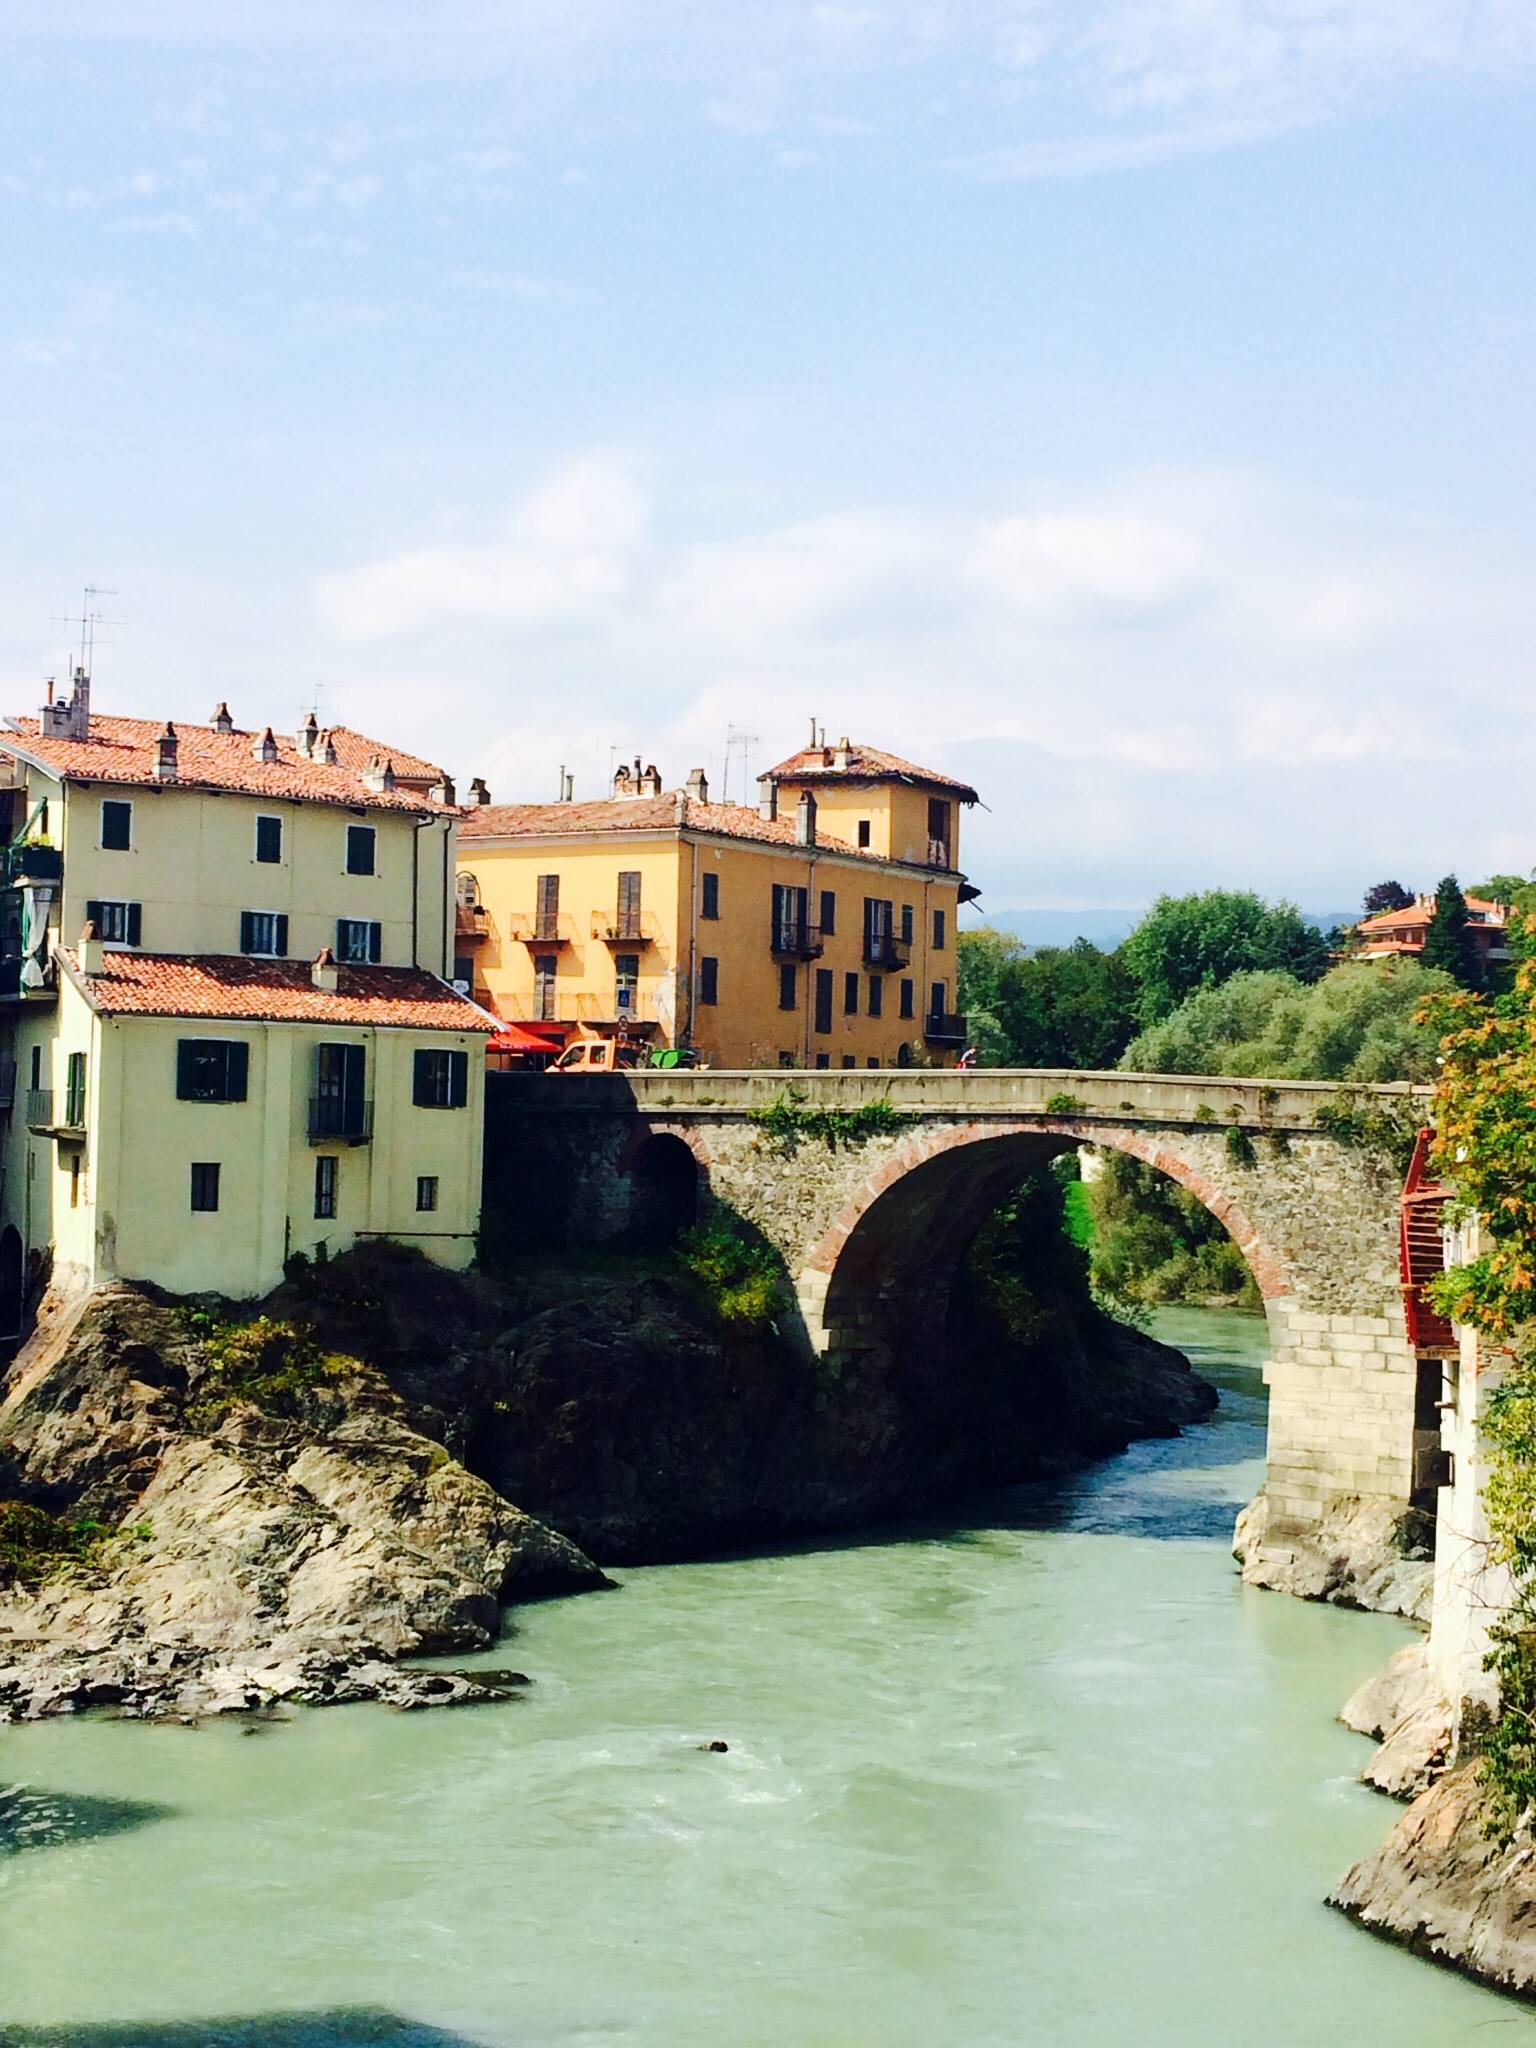
\includegraphics[width=.9\textwidth]{Ivrea}
\end{minipage}
\endslide
\chapter{软件环境}{安装软件}
Arduino 主页:  \url{https://www.arduino.cc}

\begin{itemize}
    \item 下载安装包
    \item 解压、安装
    \item 安装驱动
\end{itemize}
\endslide

\slide{认识软件环境}
\begin{itemize}
    \item 设置环境: 字体大小、编辑器行号、...
    \item 新建/打开\alert{项目}
    \item \alert{编译}: 检查语法, 转换成机器语言
    \item 端口: COMx (Mac 可能是  /dev/ttyserialxx,...)
    \item 上传: 把\alert{机器码}传到目标系统上并运行
    \item 保存项目
\end{itemize}
\endslide

\slide{什么是程序}
\begin{itemize}
    \item \alert{程序}是为了实现一个特定的目标而设计的一组可操作的工作步骤.
    \item 对于计算机而言, 程序就是计算机可以识别的一组有序的指令, 
        计算机根据这组指令完成相应的动作.
    \item 计算机是电子设备, 目前还不能直接听懂人的自然语言;
    \item 工程师设计了不同的计算机语言, 每一种语言遵循不同的语法规则;
    \item 程序员遵照语法规则书写源程序, 再由一个特殊的程序把它翻译成
        电子语言 (0/1、高/低\alert{电平}), 提供给计算机执行.
\end{itemize}
\endslide

\slide{怎样写好程序}
一个好的程序,除了保证功能正确、可靠以外,还应该具备:
\begin{itemize}
    \item 性能优良 (程序员的知识面、编程能力)
    \item 可读性  (良好的编程习惯)
    \item 易于维护 (编程能力、编程习惯)
    \item 兼容性/可移植性 (标准化)
\end{itemize}
\endslide


\slide{程序结构}
~\ \vskip-6mm
\begin{lstlisting}
int x;                  // 声明全局变量
void setup () {         // 初始化函数
    /*
       注释
       注释~注释~注释~注释~注释
    */
    x = 5;              // 赋值语句
    Serial.begin(9600); // 函数调用, 初始化串口
}
void loop () {          // 重复函数
    Serial.println("Hello!");  // 打印
    x = x + 1;
    delay(5000);        // 函数调用, 等待5秒
    delayMicroseconds(10);   // 更精细的等待
}
\end{lstlisting}
\endslide

\slide{串口监视器设置}
\begin{center}
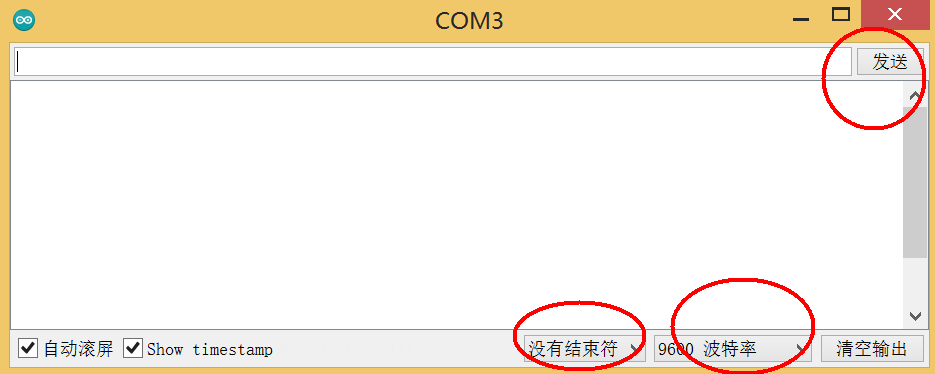
\includegraphics[width=.8\textwidth]{serial}
\end{center}

``\alert{波特率}''设置与函数 Serial.begin() 中的数值一致.

``\alert{发送}''窗口中的字符通过键盘的回车或者点击``发送'' 送往arduino板.

选择 ``\alert{没有结束符}'', 接收方只接收可见字符.
\endslide

\slide{C/C++语言基本规则}
Arduino 开发环境使用 C/C++ 编程语言. 程序语言由低到高有如下层次:
\begin{itemize}
    \item 常数、变量及其运算构成\alert{表达式};
    \item 表达式的运算结果形成一个\alert{语句};
    \item 一组语句完成一个特定功能, 可形成一个\alert{函数};
    \item 一组相关功能的函数, 可组成一个\alert{库}, 便于使用.
    \item 函数和库构成一个项目
\end{itemize}
\endslide


\slide{控制引脚电压}
\begin{center}
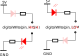
\includegraphics[width=.6\textwidth]{pincontrol}
\end{center}
本课程统一采用下一组控制方式 (\alert{HIGH}: 点亮, \alert{LOW}: 熄灭).
\endslide

\slide{程序}
~\ \vskip-6mm
\begin{lstlisting}
/*
  控制板载LED
*/
void setup () {
    pinMode(LED_BUILTIN, OUTPUT);
}

void loop () {
    digitalWrite(LED_BUILTIN, HIGH);
    delay(1000);
    digitalWrite(LED_BUILTIN, LOW);
    delay(1000);
}
\end{lstlisting}
\endslide

\slide{词汇}
\begin{itemize}
    \item[-] int (integer): 整数类型
    \item[-] delay: 延迟
    \item[-] loop: 回环, 循环
    \item[-] LED (light-emitting diode): 发光二极管
    \item[-] serial: 串行的 
    \item[-] digital: 数字化的, 用 0 和 1 表示的量
    \item[-] built-in: 内建的
\end{itemize}
\endslide

\slide{思考题}
\begin{itemize}
    \item 下面哪个是程序?
    \begin{enumerate}
        \item 按步骤完成的工作
        \item 完成工作的步骤
    \end{enumerate}
    \item 计算机能理解什么样的语言?
    \begin{enumerate}
        \item 无语法错误的英文语句
        \item 按规定格式书写的程序语句 
        \item 由高低电压组成的电信号
    \end{enumerate}
    \item 如果串口控制器的波特率设置和arduino程序设置不一致,
        会发生什么现象? (自己尝试一下)
\end{itemize}
\endslide


\slide{任务}
模仿心跳:

快闪两次, 间隔0.2秒, 熄灭0.6秒 (大致相当于每分钟60次)
\endslide

\chapter{认识Arduino}{认识Arduino}

\centering
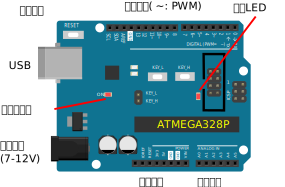
\includegraphics[width=.8\textwidth]{ArduinoC}
\endslide

\slide{控制板载LED}
\begin{minipage}[c]{.3\textwidth}
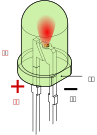
\includegraphics[width=\textwidth]{LED}
\end{minipage}
\begin{minipage}[c]{.68\textwidth}
\alert{LED} (发光二极管) 两端加正向电压, 内部发光材料被激发发光.

控制发光二极管工作步骤:
\begin{enumerate}
    \item 选定控制 LED 的引脚 (端口): 一端选定固定电压(通常是\alert{地}),
        另一端选定一个可控制的引脚;
    \item 可控制的引脚设置成输出功能;
    \item 在可控引脚上输出电压 (高或低)
\end{enumerate}
\end{minipage}
\endslide

\chapter{外接设备}{面包板}
\centering
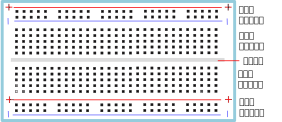
\includegraphics[width=.7\textwidth]{breadboard}

%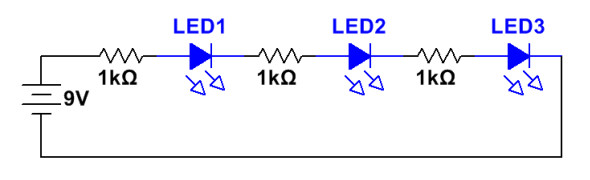
\includegraphics[width=.6\textwidth]{ledsketch}
\endslide

%\slide{面包板}
%\centering
%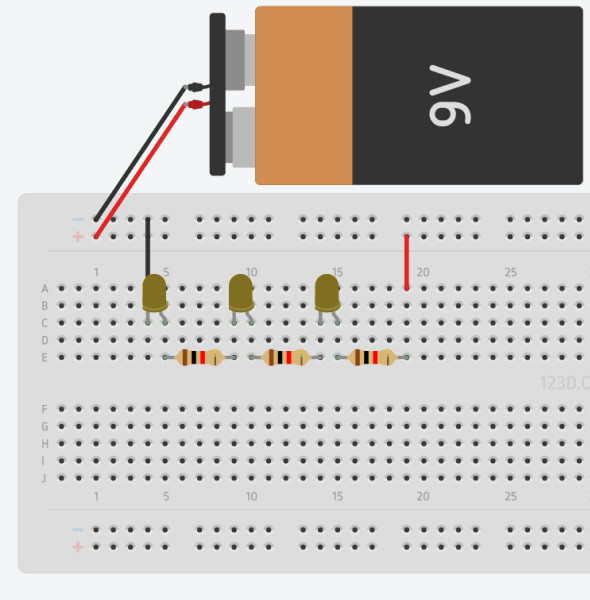
\includegraphics[width=.6\textwidth]{poweredled}
%\endslide
%

\slide{连外接LED}
\centering
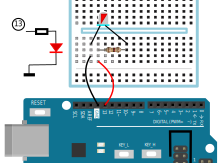
\includegraphics[width=.8\textwidth]{LED1}
\endslide


\slide{通过串口监视器控制}
~\ \vskip-6mm
\begin{lstlisting}
int pin = 12;
...
void loop () {
    char b;

    if (Serial.available()) {
        b = Serial.read();
        if (b == '0') {
            digitalWrite(pin, LOW);
        } else {
            digitalWrite(pin, HIGH);
        }
    }
}
\end{lstlisting}
\endslide

\chapter{条件语句}{条件语句--if/else}
~\ \vskip-6mm
\begin{lstlisting}[emph={do_something,do_other,do_any_other_thing}]
    if (condition1) {     // 满足条件1
        do_something();
    } else if (condition2) {   // 否则, 看条件2
        do_other();
    } else {                // 不满足以上条件
        do_any_other_thing();
    }
\end{lstlisting}
条件的产生:
\begin{itemize}
    \item 比较运算符;
    \item 逻辑运算符: 与 (\&\&),  或(||), 反 (!);
    \item 数值量本身 (常量、变量、函数调用...).
\end{itemize}
\endslide


\slide{例子}
~\ \vskip-6mm
\begin{lstlisting}[escapeinside=]
  int a = 10, b = 5, c;

  if (a > 10 || b == 5)  // 条件成立
  if (a != b)            // 条件成立
  if (a = b)             // 当 b 不为 0 时, 条件成立
  if (a == b*2)          // 条件成立
  if (a == b && false)   // 条件恒不成立
  if (1)                 // 条件恒成立
  // 只有 0 是 false, 任何非零值是 true
  c = (a != b);          // 将'a 不等于 b'的判断赋值给c
  a = !b;                // a = 0
\end{lstlisting}
运算优先级.

用括号明确运算优先级.
\endslide


\slide{条件语句--switch/case}
~\ \vskip-6mm
\begin{lstlisting}[emph={do_something,do_other}]
    switch (value) {
    case a:             // 当 value == a 时
        do_something();
        break;
    case b:             // 当 value == b 时
        do_other();
        break;
    default:            // 除了已列条件以外
        break;
    }
\end{lstlisting}
条件语句可\alert{嵌套}, 需要注意嵌套层次! 
\endslide

\slide{忙等待}
~\ \vskip-6mm
\begin{lstlisting}
// 函数 delay() 的可能形式
void delay (int ms) {
    int a, b;
    unsigned long total = 100*ms;
    while (total-- > 0) {
        a = a * 3;       
        b = b + a;      // 假设这两条指令耗时10us.
    }
}
\end{lstlisting}
delay()、delayMicroseconds() 靠大量执行无意义指令来消耗时间,
不是一个好的方法.
\endslide

\slide{忙等待}
~\ \vskip-6mm
\begin{lstlisting}
void loop () {             // 0: 灭, 其他: 闪
    static char b;
    if (Serial.available())
        b = Serial.read();
    if (b == '0') {
        digitalWrite(pin, LOW);
    } else {
        digitalWrite(pin, HIGH);
        delay(1000);
        digitalWrite(pin, LOW);
        delay(1000);
    }
}
\end{lstlisting}

在闪烁时, 如果要LED熄灭, 最坏的情况要等2秒以后. 
\endslide

\slide{改进的方法}
~\ \vskip-6mm
\begin{lstlisting}
void loop () {
    unsigned long now = millis();        // 获得当前时间

    if (Serial.available())
        b = Serial.read();
    if (b == '0') {
        digitalWrite(pin, LOW);
    } else if (now - previous >= 1000) {  // 如果超时
        if (state == LOW)  state = HIGH;
        else state = LOW;
        digitalWrite(pin, state);         // 改变LED状态
        previous = now;          // 记下当前时间, 以备后用
    }
}    // 此方法只作理解, 不要求掌握
\end{lstlisting}
\endslide


\slide{词汇}
\begin{itemize}
    \item[-] breadboard: 面包板, 多孔连接板
    \item[-] char (character): 字符型变量, 字节变量
    \item[-] unsigned: 无符号的 (只用于表示正数)
    \item[-] available: 可用的
    \item[-] analog: 模拟的, 用于描述连续变化的物理量(与digital 相对)
\end{itemize}
\endslide

\slide{思考题}
~\ \vskip-16mm ~
\begin{itemize}
    \item 为了让发光二极管有效工作 (既要足够亮由要防止损坏), 在5V电压
        工作环境中, 合适的限流电阻大小应该是:

       1. 10 $\Omega$ \qquad\qquad 2. 200$\Omega$ \qquad\qquad 3. 2k$\Omega$

    \item 在一组学生成绩中挑出最好(90分以上)和最差(不及格)的学生组队, 条件
        语句的用法应该是:
    \begin{enumerate}
        \item \verb|if (90 <= score < 60)|
        \item \verb!if ((score < 60) || (score >= 90))!
        \item \verb|if ((60 > score) && (score >= 90))|
        \item \verb|if (score < 60).... else if (score >= 90)|
    \end{enumerate}
    \item 用两只 digital 引脚 (如 8 和 10) 分别接LED 两端, 能否让它工作?
        两只脚应如何设置? 如果可行,试用程序实现.
\end{itemize}

\endslide
\slide{任务}
~\ \vskip-6mm 连接多个LED
\begin{center}
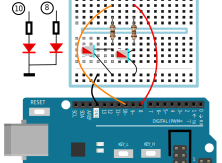
\includegraphics[width=.7\textwidth]{LED2}
\end{center}
\endslide

\slide{任务}
通过串口监视器, 用4个键 ``1''  ``2''  ``3''  ``4'' 控制2个LED:

\indent 1、2两个键控制 LED1 亮/灭,3、4两个键控制 LED2 亮/灭.....

提示:
\begin{lstlisting}
char b;
int  v;
....
    b = Serial.read();      // 读一个字符
    if (b == '1') ...
    v = Serial.parseInt();  // 读一个数字
    if (v == 2) ...
\end{lstlisting}
\endslide


\chapter{循环结构}{循环结构}
~\ \vskip-6mm
\begin{lstlisting}
int pin[] = {4, 5, 6, 7};            // 数组下标从0开始
void loop () {
    int i = 0;

    while (i < 4) {       // while / do...while 结构
        digitalWrite(pin[i], LOW);
        i = i + 1;   // i++;
    }
    delay(1000);
    // for (初始状态; 执行条件; 每次的状态改变)
    for (i = 0; i < 4; i = i + 1) {    // for 结构
        digitalWrite(pin[i], HIGH);
        delay(1000);
    }
}
\end{lstlisting}
\endslide

\slide{任务}
4个LED按下面的方式循环:

\begingroup
\fontsize{12}{8}\selectfont
\color{red}
$\bullet\circ\circ~\circ$

$\circ\bullet\circ~\circ$

$\circ\circ\bullet~\circ$

$\circ\circ\circ~\bullet$

$\bullet\circ\circ~\circ$

$\circ\bullet\circ~\circ$

$\circ\circ\bullet~\circ$

$\circ\circ\circ~\bullet$

$\bullet\circ\circ~\circ$

$\circ\bullet\circ~\circ$

......
\endgroup
\endslide

\slide{变量交换/传递}

 $val1 \rightleftharpoons val2$:
\begin{lstlisting}
    int temp;
    temp = val1; val1 = val2; val2 = temp;

    temp = pin[0];
    for (int i = 0; i < TOTAL-1; i++)
        pin[i] = pin[i + 1];
    pin[TOTAL-1] = temp;
\end{lstlisting}
\endslide


\slide{变量交换/传递}
~\ \vskip-6mm
\begin{lstlisting}
int pin[4] = {4, 5, 6, 7};     // 声明数组
int state[] = {LOW, LOW, LOW, HIGH};
\end{lstlisting}
\pause
\begin{lstlisting}
void loop () {
    int i, t;
    for (i = 0; i < 4; |\alert{i++}|) {
        digitalWrite(pin[i], state[i])
    }
\end{lstlisting}
\pause
\begin{lstlisting}
    t = state[0];
    for (i = 0; i < 3; |\alert{i++}|)
        state[i] = state[i + 1];
    state[3] = t;
    delay(1000);
}
\end{lstlisting}
\endslide

\chapter{脉冲宽度调制}{三色LED}
\centering
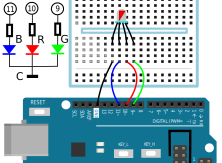
\includegraphics[width=.8\textwidth]{LED3}
\endslide

\slide{如何改变亮度}
当闪烁频率大于100Hz后, 人眼感觉不到闪烁(\alert{视觉暂留}效应)

ON/OFF 比值变化导致亮度变化

\begin{figure}
\centering
    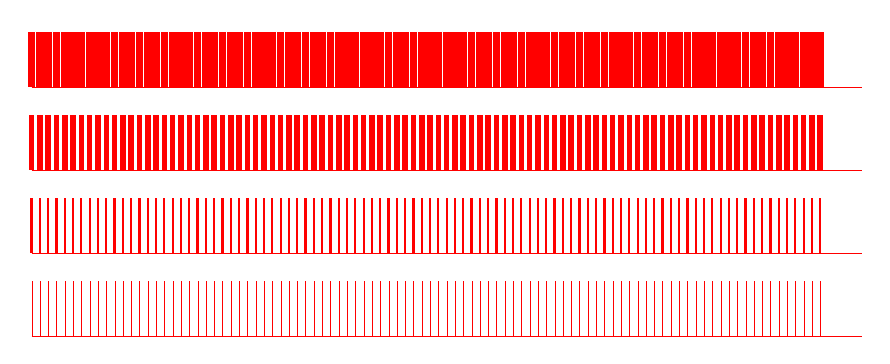
\begin{tikzpicture}[x=3pt, y=20pt]
    \foreach \x in {0,1,...,95}
      {
        \draw[red, line width=0.02pt] (\x,0)-- ++(0,1);
        \draw[red, line width=0.8pt] (\x,1.5)-- ++(0,1);
        \draw[red, line width=2.0pt] (\x,3)-- ++(0,1);
        \draw[red, line width=2.8pt] (\x,4.5)-- ++(0,1);
      }
    \foreach \x in {0, 1.5, 3, 4.5}
        \draw[red, line width=0.1pt] (0, \x)-- ++(100, 0);
\end{tikzpicture}
\end{figure}
\endslide

\slide{改变亮度的程序}
~\ \vskip-6mm
\begin{lstlisting}
int red = 10;

void setup () {
    pinMode(red, OUTPUT);
}

void loop () {
    digitalWrite(red, HIGH);
    delay(2);
    digitalWrite(red, LOW);
    delay(8);
}
\end{lstlisting}
\endslide


\slide{PWM}
\alert{PWM} (Pulse Width Modulation): 脉冲宽度调制.
\begin{figure}
\centering
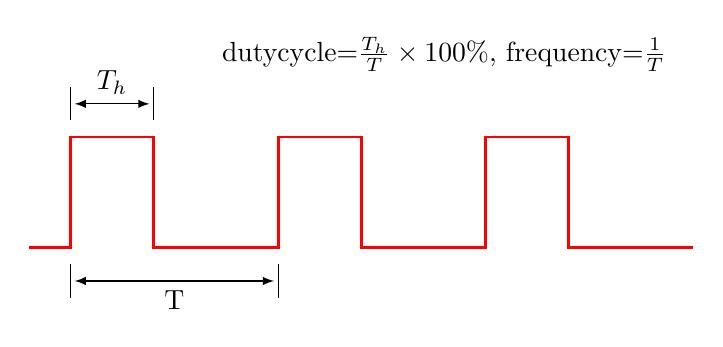
\begin{tikzpicture}[x=1.5pt,y=2pt, >=latex]
    \draw[red,line width=1pt] (0,0)-- ++(10,0)--
        ++(0,20)-- ++(20,0)-- ++(0,-20)-- ++(30,0)--
        ++(0,20)-- ++(20,0)-- ++(0,-20)-- ++(30,0)--
        ++(0,20)-- ++(20,0)-- ++(0,-20)-- ++(30,0);
    \draw[line width=0.3pt] (10,23)--(10,29);
    \draw[line width=0.3pt] (30,23)--(30,29);
    \draw[<->] (11,26)-- ++(18,0) node [midway,above] {$T_h$};
    \draw[line width=0.3pt] (10,-3)--(10,-9);
    \draw[line width=0.3pt] (60,-3)--(60,-9);
    \draw[<->] (11,-6)-- ++(48,0) node [midway,below] {T};
    \node (a) at (100,35) {dutycycle=$\frac{T_h}{T}\times 100 \%$,
       frequency=$\frac{1}{T}$};
\end{tikzpicture}
\end{figure}
PWM 的两个重要参数: 频率、\alert{占空比}(高电平占总周期时间的比值)
\endslide

\slide{变色灯}
红、绿、蓝三个颜色亮度不同的配比, 得到不同的颜色

\begin{figure}
\centering
\begin{tikzpicture}[thick,fill opacity=0.4]
    \filldraw[fill=red, line width=0.0pt] (60:1cm) circle (12mm);
    \filldraw[fill=green, line width=0.0pt] (180:1cm) circle (12mm);
    \filldraw[fill=blue, line width=0.0pt] (300:1cm) circle (12mm);
    \node[opacity=1] at (60:25mm) {红}; 
    \node[opacity=1] at (120:18mm) {黄}; 
    \node[opacity=1] at (180:25mm) {绿};
    \node[opacity=1] at (240:18mm) {青}; 
    \node[opacity=1] at (300:25mm) {蓝}; 
    \node[opacity=1] at (0:18mm) {紫}; 
\end{tikzpicture}
\end{figure}
\endslide


\slide{通过时间长度控制颜色}

\centering
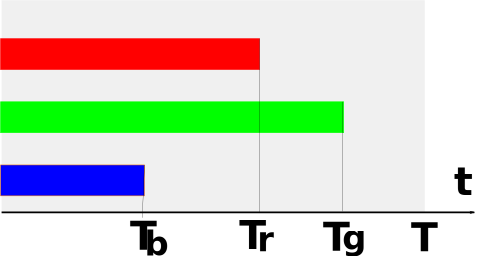
\includegraphics[width=.6\textwidth]{chrome}
\endslide

\slide{笨办法}
~\ \vskip-6mm
\begin{lstlisting}[escapeinside='']
void loop()
{    // 一个周期 20000 微秒
    int red = 1, green = 1, blue = 1;
    for (int i = 0; i < 3; i++)
        digitalWrite(pin[i], HIGH);
    time0 = micros();        // 计时开始
    while (red || green || blue) {
        now = micros();
        if ((now - time0 > Tr) && (red == 1)) {
            digitalWrite(pinR, LOW); red = 0;
        }
        ..... // 绿、蓝结构与红类似
    }
    while (micros() - time0 < '\alert{20000}') ;
}
\end{lstlisting}
\endslide

\slide{词汇}
\begin{itemize}
    \item[-] frequency: 频率
    \item[-] PWM (Pulse Width Modulation): 脉冲宽度调制
    \item[-] dutycycle: 占空比
\end{itemize}
\endslide

\slide{思考题}
~\ \vskip-16mm ~
\begin{itemize}
    \item 下面的程序有什么逻辑错误 (不考虑功能)?
\begin{lstlisting}
    int a[10], b;
    for (a[0] = 0; a[0] <= 10; a[0] = a - 2)
        b = a[a[0]];
\end{lstlisting}
    \item 下面的循环完成后, 变量 a 和 b 各是多少?
\begin{lstlisting}
    int a, b = 200;
    for (a = 20; a > 10; a = a - 2)
        b -= a;        // 此句等效于 b=b-a;
\end{lstlisting}
    \item 在 Arduino-Uno 板上, 下面的语句有什么功能性错误?
\begin{lstlisting}
    for (int pin = 0; pin < 5; pin++)
        analogWrite(pin, 128);
\end{lstlisting}

\end{itemize}
\endslide

\slide{任务}
学习使用 PWM 控制函数改变亮度:
\begin{lstlisting}
    analogWrite(pin, rate);
    // pin: 需要控制的引脚 (仅3、5、6、9、10、11 引脚可用)
    // rate: 控制占空比, 0 <= rate <= 255
\end{lstlisting}

\begin{enumerate}
    \item 红色, 由暗到亮缓慢变化;
    \item 由红转绿 (红色成份逐渐减少, 绿色成份逐渐增加).
\end{enumerate}
\endslide


\slide{蜂鸣器}
\begin{itemize}
    \item 使用PWM控制蜂鸣器--- analogWrite() 不能改变频率, 
        只能改变占空比,  占空比影响声音大小;
    \item tone() 改变频率, 占空比 50\% (不要求PWM引脚, 但每次只能用1只脚).
\end{itemize}

\begin{lstlisting}
    tone(pin, frequency);
    tone(pin, frequency, duration);
    // pin: 引脚号
    // frequency: 频率 (Hz)
    // duration: 持续时间 (ms)
    // C++ 允许同一个函数设计不同形式的调用参数
    noTone(pin);      // 停止发声
\end{lstlisting}
\endslide

\chapter{输入}{按键}
\centering
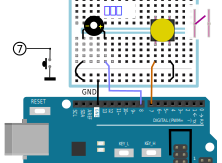
\includegraphics[width=.8\textwidth]{key}
\endslide

\slide{读按键方法}
~\ \vskip-6mm
\begin{lstlisting}
void setup () {
    pinMode(pin1, INPUT);
    pinMode(pin2, INPUT_PULLUP);
}
void loop () {
    int button;
    button = digitalRead(pin1);
    if (button == HIGH) {       // pin1 按下
        ........
    }
    button = digitalRead(pin2);
    if (button == LOW) {        // pin2 按下
        ........
    }
}
\end{lstlisting}
\endslide

\slide{板载按键}
~\ \vskip-6mm
板载两个按键 KEY\_H和KEY\_L 结构略有不同: KEY\_H 按下时, 引脚是高电平;
KEY\_L按下时, 引脚是低电平.

\begin{center}
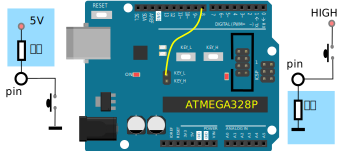
\includegraphics[width=.76\textwidth]{onboardkey}
\end{center}
常态为高电平的输入控制信号, 设置引脚输入功能 \\
pinMode(pin, \alert{INPUT\_PULLUP})
\endslide

\slide{任务}
\begin{enumerate}
    \item 使用按键控制板载LED: KEY\_H 点亮, KEY\_L 熄灭.

    \item 用按键控制蜂鸣器, 有按键时, 发出三次短促的500Hz声音.
\end{enumerate}
\endslide

\slide{任务}
用蜂鸣器输出一个音阶. 音阶频率:

440, 494, 554, 587, 659, 740, 831, 880
\endslide

\chapter{数码管}{8段数码管}\label{page:led8}
一个 8 段\alert{数码管}由8个LED组成, 通过编程点亮不同的LED, 产生不同的字形.

\begin{center}
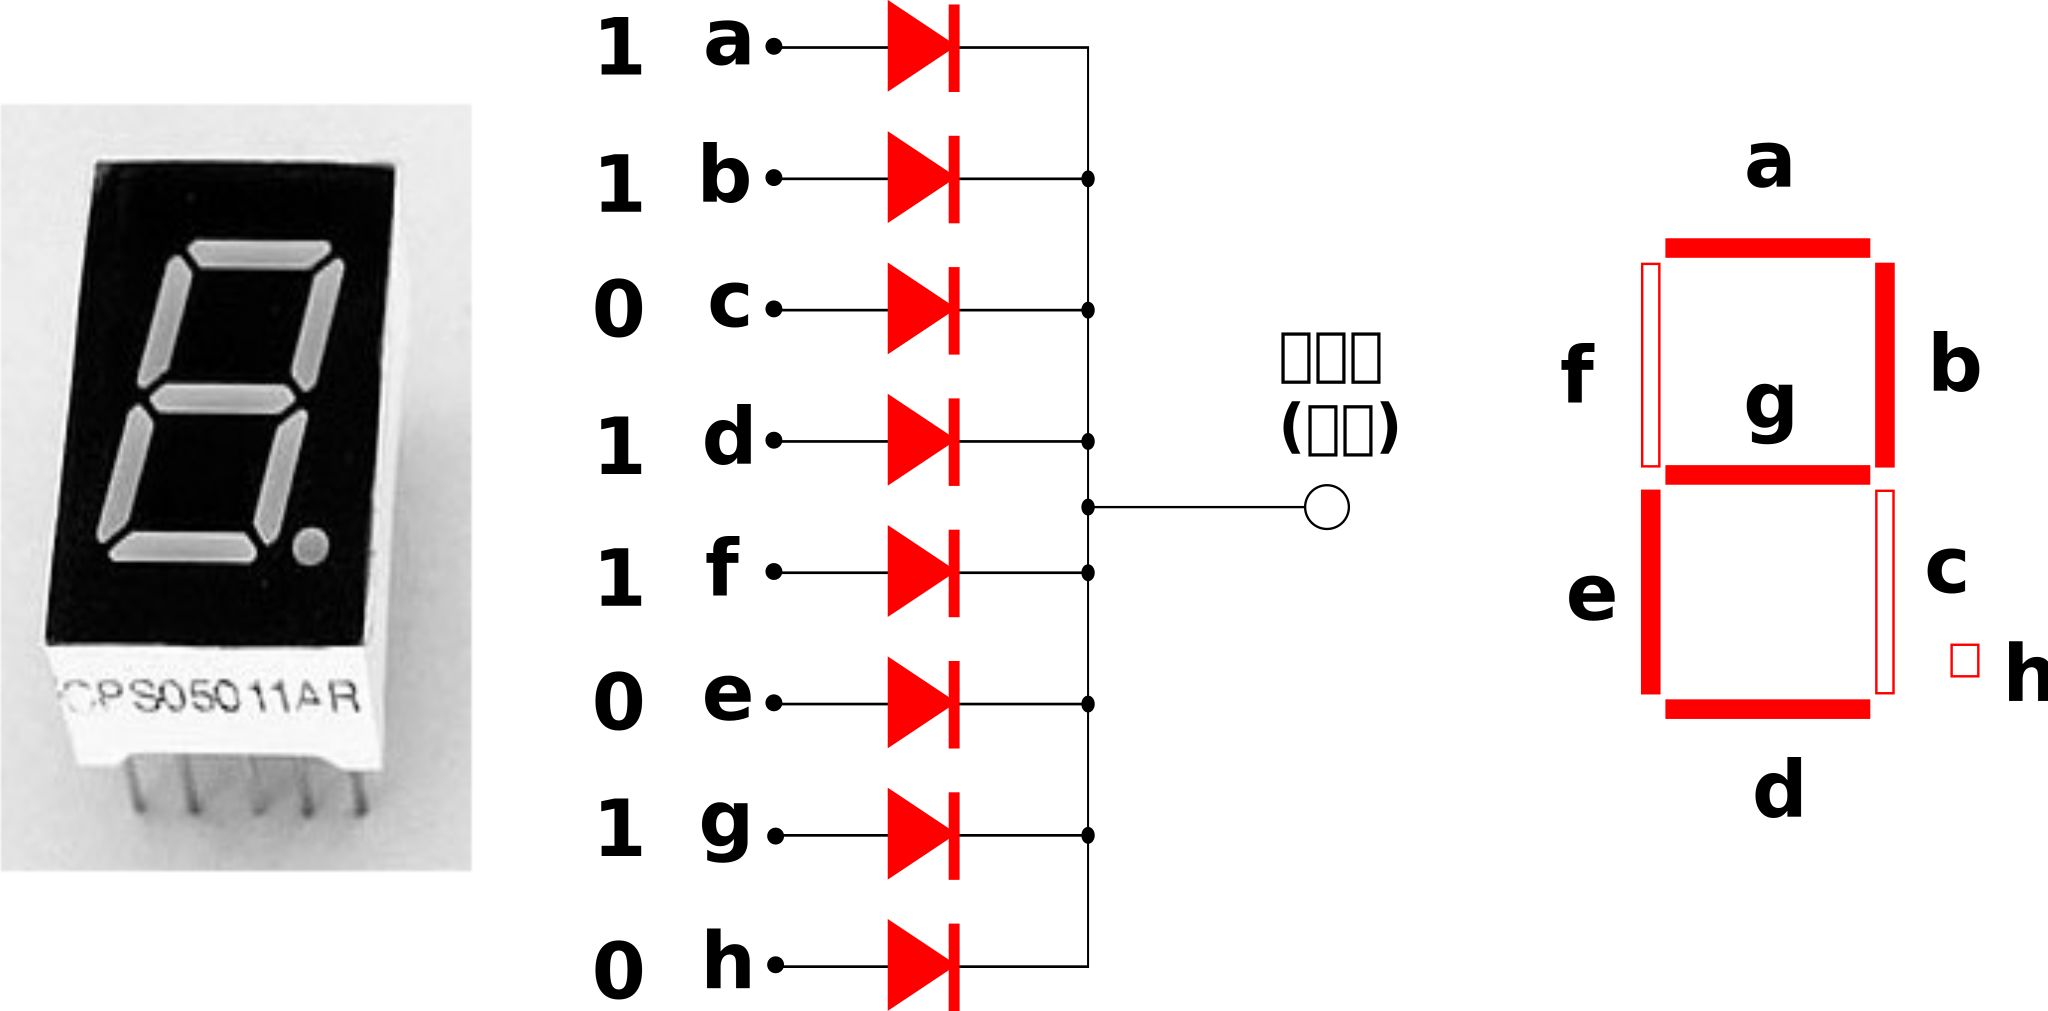
\includegraphics[width=.7\textwidth]{led8}
\end{center}
一个8段数码管有10个引脚 (8个LED控制端,1个公共端, 1个空引脚).
\endslide

\slide{多位数码管}
为了减少数码管的外接引脚, 用\alert{串行}方式输入编码, 内部转换成\alert{并行}.
\ \\
\begin{center}
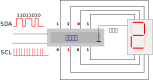
\includegraphics[width=.75\textwidth]{converter}
\end{center}
\endslide

\slide{4位数码管}
\centering
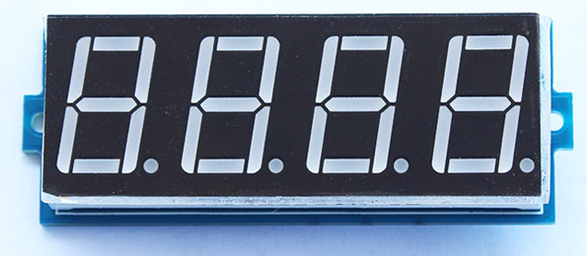
\includegraphics[width=.5\textwidth]{led4_front}

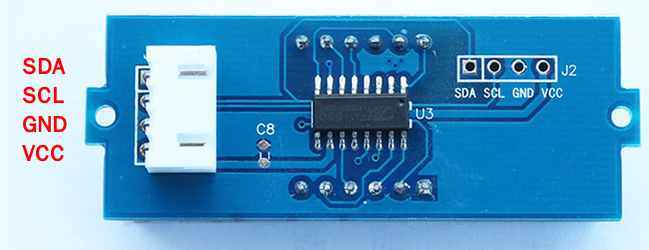
\includegraphics[width=.53\textwidth]{led4_back}
\endslide

\slide{4位数码管}
\centering
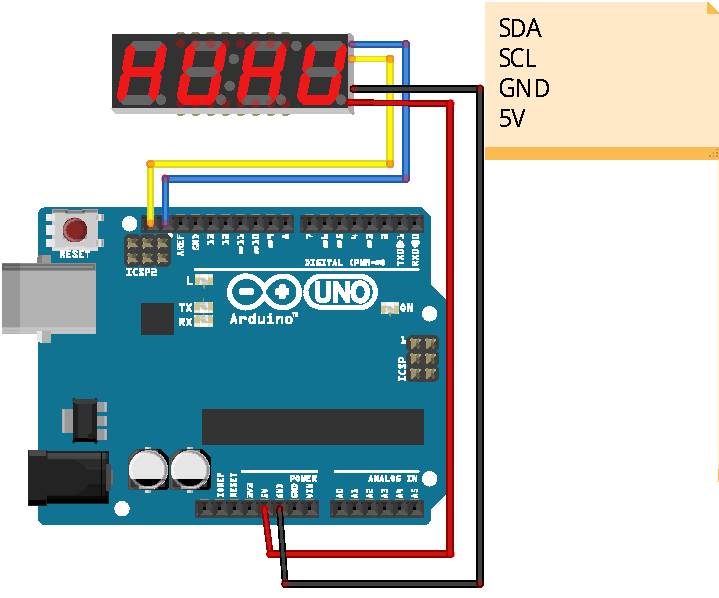
\includegraphics[width=.6\textwidth]{seg8_led}
\endslide

\slide{使用数码管库}
添加库的几种方法
\begin{enumerate}
    \item 集成开发环境的库管理, 关键字搜索 (推荐方法);
    \item 集成开发环境的库管理添加ZIP文件;
    \item 手工解压 ZIP 文件, 将整个目录复制到 Libraries (这也是以上
        两个方法的最后效果).
\end{enumerate}
\endslide

\slide{数码管控制函数}
~\ \vskip-6mm
\begin{lstlisting}
#include <TM1650.h>

TM1650 d;           // 缺省值 4位数码管
void setup () {
    Wire.begin();
    d.init();
}
void loop () {
    d.displayOff();             // 全灭
    ...
    d.displayString("abcd");    // 显示字符串
    d.setBrightness(br);        // 亮度 0--7
    d.displayOn();              // 字符显示
    d.setDot(pos, true/false);  // 显示/消隐小数点
    ...
}
\end{lstlisting}
\endslide

\slide{思考题}
\definecolor{magentacitecolor}{rgb} {0.0, 0.0, 0.9}
~\ \vskip-16mm ~
\begin{itemize}
    \item Arduino-Uno 板上, 以下哪个引脚可以用函数 analogWrite()操作?

       1\qquad\qquad 2 \qquad\qquad 3 \qquad\qquad 4
    \item 以下哪个引脚可以用函数 tone() 操作?

       5\qquad\qquad 6 \qquad\qquad 7 \qquad\qquad 都可以
   \item 按第\pageref{page:led8}页的图, 如果要让数码管显示``5.'', abcdefgh
       对应的编码是:

        10101010 \qquad 01010101 \qquad 10110111 \qquad 01001000
    \item 引脚设置了 pinMode() 为 INPUT 后, 以下哪些方式可确保读到0?
    \begin{enumerate}
        \item 外接上拉电阻, 引脚悬空
        \item 外接下拉电阻, 引脚悬空
        \item 无上拉/下拉电阻, 引脚悬空
        \item 无上拉/下拉电阻, 引脚接地
    \end{enumerate}

\end{itemize}
\endslide

\slide{任务}
\begin{enumerate}
    \item 下面的程序片将 1 位数字填入字符串的首位. 试用4位数码管
        循环显示0--9 十个数字, 每次间隔1秒 (简单的秒计数器).
\begin{lstlisting}
    char *s = "    ";       // 4个空格
    i = 4;                  // i 是待显示的数字
    s[0] = i + '0';
    d.displayString(s);     // 显示字符串 "4___"
\end{lstlisting}

    \item 在 Arduino 开发环境的库管理工具中, 找到 DHT-sensor-library 并安装.
\end{enumerate}
\endslide

\slide{设计函数}
~\ \vskip-6mm
\begin{lstlisting}
char *str = "1234";         // 全局变量. C++会有警告.
// 函数声明格式: 返回值类型 函数名(形式参数列表)
char *convert(long int t) {
    char rem = 0;           // 局部变量

    for (int i = 3; i >= 0; i--) {
        rem = t % 10;
        str[i] = rem + '0'; // 把数字转换成字符
        t = t / 10;         // also:  t /= 10;
    }
    return str;             // 返回值
}
\end{lstlisting}
\endslide

\slide{任务}
设计一个秒表, 格式``12.34'' (精度到0.01s), 用数码管显示计时.
\begin{lstlisting}
    now = millis();     // 获得系统运行到当前的毫秒数
\end{lstlisting}
\pause
提示:
\begin{lstlisting}
    now = millis();     // 获得系统运行到当前的毫秒数
    now = now / 10;     // 保留到百分之一秒
    ......              // 把数字转换成字符串
    d.displayString(str);
    d.setDot(1, true);  // 秒单位, 2位小数
\end{lstlisting}
\endslide

\chapter{温度/湿度传感器}{DHT11}

DHT11 (Digital Humidity Temperature), 数字温湿度传感器,
串行数字输出.

温度范围 0--50$^\circ$C, 精度 0.1$^\circ$C

湿度范围 20/30--80/90\% (与温度条件有关), 精度 1\% 
\endslide


\slide{电路连接}
\centering
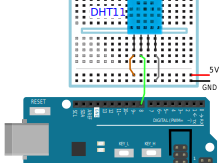
\includegraphics[width=.8\textwidth]{temperature}
\endslide

\slide{DHT 库}
~\ \vskip-6mm
\begin{lstlisting}
// DHT-sensor-library
#include <DHT.h>

DHT dht(pin, DHT11);
    ...
    dht.begin();

    delay(2000);            // 转换比较慢,每次读数需要等待
    float h = dht.readHumidity();
    float t = dht.readTemperature();        // 摄氏温度
    float f = dht.readTemperature(true);    // 华氏温度
    // 华氏/摄氏温度转换: f = t*1.8+32
\end{lstlisting}
\endslide


\slide{词汇}
\begin{itemize}
    \item[-] library: 图书馆,(软件)库
    \item[-] function: 函数, 功能
    \item[-] sensor: 传感器
    \item[-] humidity: 潮湿度
    \item[-] temperature: 温度
\end{itemize}
\endslide

\slide{思考题}
\begin{itemize}
    \item 当声明 \verb|int a=5, b=6;| 时, 以下哪个运算结果的数值最大?

        10*a/b\qquad\qquad a/b*10 \qquad\qquad 10/b*a\qquad\qquad 10.0*a/b
    \item 对于C语言来说, 函数的形式参数和实际调用参数

    数量必须一致\qquad\qquad  类型必须一致\qquad\qquad 数量、类型都要一致

    \item 函数 \verb|micros()| 返回无符号长整形格式(unsigned long int,
        32位二进制), 经过约多长时间后这个数字会溢出?

    1个小时\qquad\qquad\ 10个小时\qquad\qquad 2天 \qquad\qquad 50天
\end{itemize}
\endslide


\slide{任务}
\begin{enumerate}
    \item 设计一个函数 \verb|float CtoF(float t)|, 用来转换摄氏--华氏温标;
    \item 配合数码管显示设备, 即时显示温度/湿度;
    \item 用按键切换显示功能 (每按一次, 交替显示温度或湿度).
\end{enumerate}
\endslide


\chapter{灯带}{灯带原理}
\begin{itemize}
    \item 灯带由一组前后串联的三色发光二极管构成;
    \item 每一个发光二极管有一个控制芯片, 输出红、绿、蓝三色强度;
    \item 红、绿、蓝各由8位码控制, 每写入24位, 数据向下一个LED推进.
\end{itemize}
\begin{center}
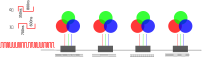
\includegraphics[width=.9\textwidth]{stripe}
\end{center}
\endslide

\slide{灯带函数}
~\ \vskip-6mm
\begin{lstlisting}[morekeywords={uint32_t}]
#include <Adafruit_NeoPixel.h>

  Adafruit_NeoPixel strip(
      LED_COUNT,            // 灯珠数目
      LED_PIN,              // 控制引脚 (PWM)
      NEO_GRB + NEO_KHZ800  // 灯带类型
      );

  strip.begin();            // 初始化

  strip.setBrightness(br);  // 亮度 (0--255)
  uint32_t color = strip.Color(R,G,B);   // 灯珠颜色
  strip.setPixelColor(pixel, color);
  strip.show();             // 数据生效
  strip.clear();            // 全灭
\end{lstlisting}
\endslide


\slide{任务}
白线接arduino的 GND, \colorbox{red}{\color{blue}{+5V}} (红线) 接
arduino的 5V, \colorbox{green}{\color{black}{Di}} (绿线)
接 arduino的 某个PWM引脚.
\begin{enumerate}
    \item 1--10: 红色, 11--20: 绿色, 21--30: 蓝色
    \item 逐次点亮从1--30灯珠, 间隔0.1秒
\end{enumerate}

\begin{minipage}[t]{0.1\textwidth}
~~~~
\end{minipage}
\begin{minipage}[t]{.4\textwidth}
    \fontsize{12}{12}\selectfont\color{red}
$\bullet\circ\circ\circ\circ\circ\circ\circ\circ\circ\circ...$

$\circ\bullet\circ\circ\circ\circ\circ\circ\circ\circ\circ...$

$\circ\circ\bullet\circ\circ\circ\circ\circ\circ\circ\circ...$

$\circ\circ\circ\bullet\circ\circ\circ\circ\circ\circ\circ...$

......
\end{minipage}
\begin{minipage}[t]{.4\textwidth}
    \fontsize{12}{12}\selectfont\color{red}
$\bullet\circ\circ\circ\circ\circ\circ\circ\circ\circ\circ...$

$\bullet\bullet\circ\circ\circ\circ\circ\circ\circ\circ\circ...$

$\bullet\bullet\bullet\circ\circ\circ\circ\circ\circ\circ\circ...$

$\bullet\bullet\bullet\bullet\circ\circ\circ\circ\circ\circ\circ...$

......
\end{minipage}
\endslide

\slide{流光溢彩}
尝试 Adafruit\_NeoPixel 库中的例子.

\begin{center}
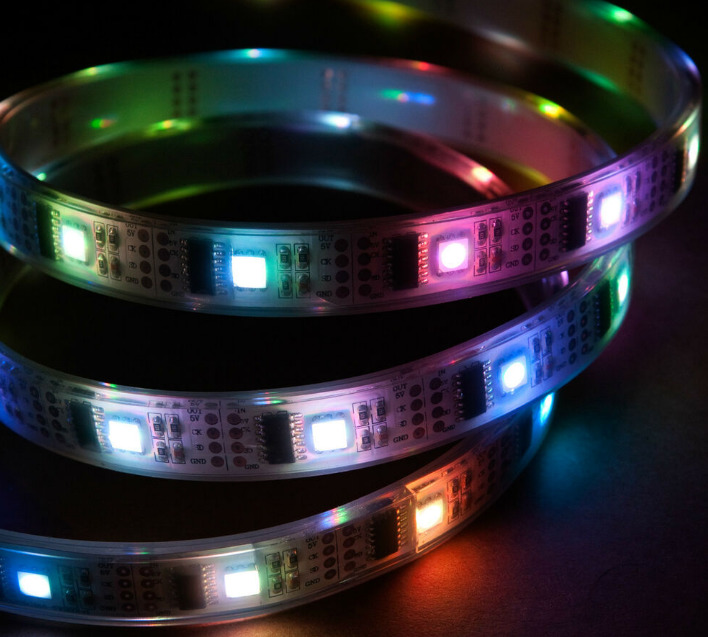
\includegraphics[width=.4\textwidth]{colorful}
\end{center}
\endslide


\slide{词汇}
\begin{itemize}
    \item[-] stripe: 条带
    \item[-] pixel: 点像素
    \item[-] HSV (Hue, Saturation, Value): HSV 色彩空间 (色调、饱和度、明亮度)
\end{itemize}
\endslide


\slide{思考题}
\begin{itemize}
    \item 控制灯带中某个灯珠的亮度(白色), 最多能有几级?

    8\qquad\qquad 256 \qquad\qquad 511\qquad\qquad 255$\times$255+1
    \item 以现有灯带的设定, 假设写入灯带数据线的每一位``0''、``1'' 编码
        平均时间是1200ns, 完成30个灯珠的操作最短时间是多少?
        (灯带很长时, 需要考虑操作的时间效果。这个问题的意义就在于此。)

    36$\mu$s \qquad\qquad 28.8$\mu$s \qquad\qquad 864$\mu$s \qquad\qquad 1ms
\end{itemize}
\endslide

\setcounter{slidesection}{-1}

\slide{知识点小结}
\begin{itemize}
    \item 建立程序设计思想
    \item 理解计算机是如何工作的
    \item 学习简单设备的控制方法
\end{itemize}
\endslide

\end{document}
